\section{Introduction}
Hotel booking cancellations create uncertainty about how much reserved demand will become realised demand. A room released close to arrival may be difficult to resell, while staffing and other resources may already have been planned. A cancellation score can help prioritise booking confirmation and capacity review, but a useful analysis also needs to explain what the score measures, how it was evaluated, and which decisions the evidence can support.

This project combines the group's data preparation, exploratory analysis, K-means segmentation, baseline classification, ensemble modelling, explanation, and probability assessment into one analytical workflow. The aim is to compare predictive approaches under common inputs and evaluation definitions, then relate the resulting patterns to possible hotel decisions. Model comparison alone is insufficient: a high score on randomly held-out records can coexist with weaker performance on new booking profiles or a later arrival period.

We address four questions. \textbf{RQ1:} How well do the selected retrospective booking attributes discriminate cancellations under a shared holdout protocol? \textbf{RQ2:} Which attributes contribute to the fitted model's predictions? \textbf{RQ3:} How do cancellation patterns vary across hotel types and numerical booking segments? \textbf{RQ4:} How do calibration, threshold choice, and evaluation limitations affect the interpretation of operational recommendations? These questions preserve the proposal's predictive and explanatory aims while narrowing its initial-booking claim: the published data do not establish the timestamp at which every retained field became available.

Our contribution is an aligned comparison with traceable predictions and robustness checks. Segmentation describes booking combinations, classifiers predict cancellation, SHAP explains the fitted forest, and calibration assesses its scores. Neither a cluster label nor a feature attribution demonstrates an intervention effect.

\section{Data and Preparation}
\subsection{Source and Analytical Population}
The Hotel Booking Demand data describe bookings at a city hotel and a resort hotel in Portugal, with scheduled arrivals from July 2015 to August 2017 \citep{antonio2019}. The combined CSV contains 119,390 records and 32 columns. We retain the public source file alongside the cleaned file so that transformations can be traced. The binary target is \texttt{is\_canceled}: 1 denotes cancellation and 0 denotes a booking that was not cancelled. The target is not a measured financial loss or a cancellation time.

The cleaning rules leave 118,564 records, a reduction of 826. The final file has no missing values and contains 44,176 cancellations and 74,388 non-cancellations. Table~\ref{tab:data} gives the main sample counts. We preserve a unique \texttt{row\_id} for matching data, folds, predictions, and diagnostic outputs. It is excluded from every predictive input matrix.

\begin{table}[t]
\caption{Cleaned data and fixed evaluation populations. Cancellation rates are calculated from unrounded counts.}
\label{tab:data}
\centering
\begin{tabular}{lrr}
\toprule
Population & Bookings & Cancelled (\%)\\
\midrule
All cleaned data & 118,564 & 37.26\\
City Hotel & 78,899 & 41.91\\
Resort Hotel & 39,665 & 28.01\\
Random training & 94,851 & 37.26\\
Random test & 23,713 & 37.26\\
Earlier-arrival training & 96,428 & 36.48\\
Later-arrival test & 22,136 & 40.64\\
\bottomrule
\end{tabular}
\end{table}

\subsection{Cleaning and Feature Construction}
We fill missing children with zero and replace missing country and agent entries with an explicit unknown category. Agent is a categorical code, not an ordered numerical measurement. The highly incomplete company field is removed. Records with a zero guest count, a zero-night stay, or a negative average daily rate (ADR) are excluded under the predefined data-quality rules. The respective counts are 180, 715, and one, with overlapping conditions giving 826 excluded records. The rules are applied deterministically before the shared split; no quantile or scaling statistic is fitted on all records for supervised prediction. These exclusions define the study population and can also remove unusual legitimate bookings, a limitation of a rule-based cleaning policy.

We derive total guests as adults plus children plus babies, total nights as weekend nights plus weekday nights, a family indicator from the presence of children or babies, a lead-time band, and an arrival-season category. The last category is available for descriptive analysis but excluded from the common classifier. Derived fields share information with their components, so individual coefficients and attributions require care. The cleaned file retains 32 columns after removals and additions; this count includes the target, identifier, descriptive fields, and 24 supervised inputs.

We do not automatically delete identical-looking records. There is no true reservation identifier in the anonymised source, so matching records may represent separate reservations. The original raw file has 31,994 duplicate rows under its original columns, while the cleaned file has 33,985 duplicates when the artificial identifier is ignored. These are different definitions and should not be interpreted as the same count. Later analyses explicitly assess repeated 24-input profiles across evaluation partitions.

\subsection{Common Predictors and Availability}
The common classifier uses 15 numerical inputs and nine categorical inputs. Numerical inputs cover lead time, arrival-year/week/day, weekend and weekday nights, adults, children, babies, repeat-guest status, past cancellations, past non-cancelled bookings, total guests, total nights, and the family indicator. Categorical inputs are hotel, arrival month, meal, country, market segment, distribution channel, reserved room type, agent, and lead-time band.

We exclude direct outcome fields (reservation status and its date), fields that can change after booking (booking changes, assigned room type, and waiting-list days), company, and the common protocol's additional exclusions: ADR, customer type, deposit type, special requests, arrival season, and requested parking spaces. A field retained for EDA is therefore not automatically a classifier input. This distinction prevents an attractive descriptive association from silently changing the main model comparison.

Parking deserves explicit discussion. All 7,393 cleaned records requesting at least one parking space are non-cancellations; 7,360 request exactly one space. This near-deterministic pattern motivates precautionary exclusion, but does not itself establish when the field was recorded. The source construction refers to booking records reconstructed before arrival rather than guaranteed initial-booking snapshots \citep{antonio2019}. Removing parking and obvious outcome fields reduces risk without proving that every remaining attribute was available at the intended decision time.

\subsection{Preprocessing and Partitioning}
Numerical features are standardised and categorical features are one-hot encoded, with categories below 50 training occurrences pooled by the shared encoder. Unknown categories are handled by that encoder. We clone the unfitted preprocessing template within each model pipeline and fit it separately in each training fold. Standardisation is especially relevant to logistic regression and is retained for all classifiers to preserve the common representation. The random-training template produces 221 encoded features; that number may change with a different fitting population.

The primary split is stratified 80/20 with seed 42. Five fixed stratified folds partition only the 94,851 random-training records. We verify fold membership by \texttt{row\_id}, rather than trusting positional alignment across exports. The supplementary scheduled-arrival split trains through 30 April 2017 and tests on May--August 2017. Its cutoff was selected from prespecified month-ends using sample balance and coverage, not predictive performance. Random-test labels are not used to fit preprocessing, tune classifiers, fit calibration maps, or choose thresholds.

\section{Exploratory Analysis and Segmentation}
\subsection{Descriptive Cancellation Patterns}
The full cleaned dataset has a cancellation rate of 37.26\%; City Hotel's rate is 41.91\% compared with 28.01\% for Resort Hotel. Figure~\ref{fig:eda} also describes cancellation by lead-time band. This analysis describes the supplied population, including held-out records, and is not an independent validation experiment. The model feature list and fixed partitions are retained while exploratory associations are reported.

Deposit type illustrates why association must be distinguished from a recommendation. Non-refundable bookings have 14,494 cancellations among 14,587 records (99.36\%), whereas bookings without a deposit have 29,646 cancellations among 103,815 records (28.56\%). These conditional rates can reflect booking policies, group arrangements, coding conventions, or selection into contract types. They do not imply that imposing a non-refundable deposit causes cancellation. Deposit type is excluded from the shared classifier, and the analysis does not estimate the effect of changing a contract.

\begin{figure}[t]
\centering
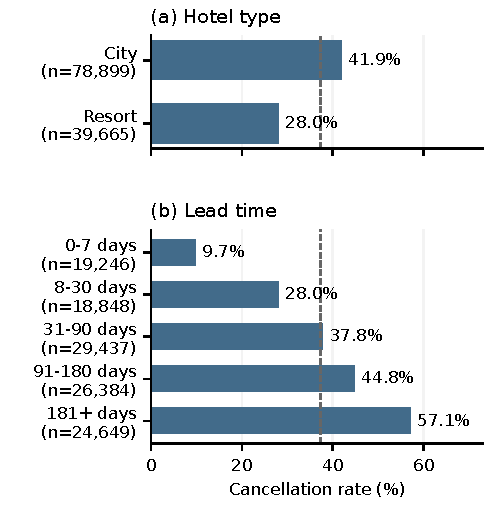
\includegraphics[width=\columnwidth]{eda_hotel_lead.pdf}
\caption{Descriptive cancellation patterns in the full cleaned data. Dashed lines mark the overall rate of 37.26\%. Hotel and lead-time comparisons are associations rather than intervention effects.}
\label{fig:eda}
\end{figure}

\subsection{Training-Only K-Means}
We cluster numerical booking attributes to obtain an interpretable segmentation separate from supervised prediction. The five inputs are lead time, total nights, total guests, ADR, and \(\log(1+\text{previous cancellations})\). ADR is justified here as a segment descriptor even though it is outside the main classifier. Cancellation, country, and the row identifier do not form the clusters.

Outlier caps are learned from random training only: ADR 252, total guests 4, lead time 476 days, and total nights 14. The transformed inputs are standardised using training statistics. K-means is fitted to training records and then assigns the test records to the nearest learned centroid. Full-data profiles combine these assignments after fitting; they do not indicate that the model was fitted on the test set.

We compare alternative cluster counts. A three-cluster solution has silhouette 0.3165, compared with 0.3032 for the retained five-cluster solution. For five clusters, fits with alternative random seeds have adjusted Rand agreement of 0.9933--0.9960 relative to seed 42 in the training stability check. We retain five clusters for the more detailed, stable description; we do not call it the silhouette-optimal choice or a proven natural partition. Cluster numbers are arbitrary identifiers, and descriptive names are assigned from the fitted profiles, not their cancellation rates.

\begin{table}[t]
\caption{Five-cluster profiles. Counts and rates summarise the full cleaned population after training-only fitting; means use original, uncapped units.}
\label{tab:clusters}
\centering
\begin{tabular}{lrrrr}
\toprule
Cluster & \(n\) & Lead days & Nights & Cancel \%\\
\midrule
0 & 59,941 & 45.7 & 2.47 & 28.45\\
1 & 18,144 & 76.1 & 3.59 & 35.95\\
2 & 19,747 & 262.8 & 3.06 & 51.32\\
3 & 14,327 & 126.9 & 8.23 & 32.04\\
4 & 6,405 & 197.0 & 2.65 & 91.73\\
\bottomrule
\end{tabular}
\end{table}

The largest cluster comprises shorter-lead, shorter-stay bookings. Cluster 1 has a mean party size of 2.91 and ADR of 175.83, compared with party sizes below two and ADR near 76--92 in most other clusters. Cluster 2 concentrates longer lead times, while cluster 3 separates long stays. Cluster 4 has mean prior cancellations of 1.61, alongside its much higher observed cancellation rate. These summaries do not mean that every member has the average characteristics.

Hotel composition changes some pooled comparisons. Long-stay bookings have a lower overall cancellation rate than the higher-ADR/larger-party segment (32.04\% versus 35.95\%), but within City Hotel this order reverses (41.62\% versus 36.54\%). Within Resort Hotel the corresponding rates are 27.40\% and 35.00\%. The long-stay segment is disproportionately Resort Hotel (67.3\%), so an overall segment ranking should not be interpreted as a common ranking within both hotels.

The random-test segment rates are 28.63\%, 36.18\%, 51.56\%, 30.14\%, and 91.87\%, with corresponding counts 11,925, 3,734, 3,910, 2,840, and 1,304. Figure~\ref{fig:clusters} compares training and test descriptions. Broad rate ordering persists in this random split, but this is not a test of future-period segment stability. Prior cancellation history was a clustering input, so the high cancellation rate in cluster 4 should not be presented as a wholly unexpected discovery.

\begin{figure}[t]
\centering
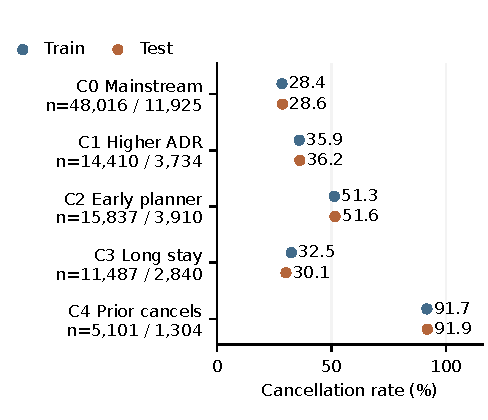
\includegraphics[width=\columnwidth]{cluster_train_test.pdf}
\caption{Cancellation rates after assigning records to training-fitted clusters; \(n\) gives training/test counts. Similar patterns describe a random split; they do not establish temporal transportability.}
\label{fig:clusters}
\end{figure}

\section{Predictive Methods and Evaluation}
\subsection{Baselines and Candidate Models}
The Dummy classifier estimates the training cancellation proportion as a constant probability. Since the proportion is below 0.50, all its decisions at threshold 0.50 are non-cancellations. Its accuracy is useful as a minimum decision baseline, while its average precision equals the evaluated cancellation prevalence when every score is tied.

Logistic regression models the log odds as a linear function of the encoded inputs with L2 regularisation. The common candidate grid varies \(C\in\{0.001,0.01,0.1,1,10,100\}\) and class weighting. We use the one-standard-error rule: among configurations within one standard error of the largest mean fold AP, choose the smallest \(C\), representing stronger regularisation. The highest mean AP is 0.796712 at \(C=100\); its standard error is 0.001229, giving an eligibility cutoff of 0.795483. The selected configuration is \(C=1\) with no class weighting (mean AP 0.796565). Its coefficients, predictions, and metrics all refer to this retained estimator.

Random forests average decision-tree predictions and can represent nonlinear interactions \citep{breiman2001}. We compare six prespecified combinations with 160 trees and seed 42, selecting by mean validation AP. The selected random-training configuration has depth 24, minimum leaf size 2, and maximum feature fraction 0.35. No class weighting is used. Its mean fold AP is 0.908, close to pooled out-of-fold AP, but those aggregations are not identical quantities.

Gradient-boosted trees sequentially add trees to improve a regularised objective \citep{chen2016}. The XGBoost experiment uses the same data, inputs, training folds, and metric definitions. We compare three configurations: depth 3 with 200 trees, depth 5 with 300 trees, and depth 7 with 300 trees, all at learning rate 0.05. Common settings are histogram tree construction, row and column subsampling of 0.85, minimum child weight 1, L2 penalty 1, and seed 42. The depth-7 configuration has the highest mean fold AP, 0.882136. The grids differ between algorithms, so results compare these specified candidates rather than an exhaustive or compute-matched search.

\subsection{Metrics and Selection Boundaries}
We report precision, recall, F1, ROC-AUC, average precision (AP), Brier score, and confusion counts with cancellation as the positive class. Precision is \(TP/(TP+FP)\), recall is \(TP/(TP+FN)\), and F1 is their harmonic mean. The baseline decision threshold is fixed at 0.50 for every classifier. Changing the threshold affects decisions and confusion counts but not the underlying ranking metrics.

The column named \texttt{pr\_auc} in the shared exports means average precision,
\begin{equation}
 \operatorname{AP}=\sum_j (R_j-R_{j-1})P_j,
\end{equation}
using scikit-learn's non-interpolated convention \citep{sklearnap}. It is not trapezoidal PR-curve area. Brier score is \(n^{-1}\sum_i(p_i-y_i)^2\), where lower is better. It reflects both calibration and discrimination, so a lower Brier score alone does not fully diagnose calibration. ROC-AUC assesses ranking across both classes; AP also depends on class prevalence.

Candidate selection and out-of-fold prediction reuse the common training folds. The selected-model validation numbers are therefore post-selection summaries, not nested-CV estimates. Similar validation and test metrics are reassuring descriptions, but do not prove the absence of overfitting, especially with repeated profiles. Alternative thresholds and calibration maps are fitted using training-derived predictions only and evaluated separately from the baseline table.

\section{Aligned Model Results}
\begin{table*}[t]
\caption{Aligned test results at threshold 0.50. AP means average precision. Shared later-arrival rows reuse randomly selected settings and are not an untouched future holdout. The separately selected forest has a different selection protocol.}
\label{tab:models}
\centering
\begin{tabular}{llrrrrrr}
\toprule
Evaluation & Model & Precision & Recall & F1 & ROC-AUC & AP & Brier\\
\midrule
Random test & Dummy & 0.000 & 0.000 & 0.000 & 0.500 & 0.373 & 0.234\\
 & Logistic regression & 0.746 & 0.651 & 0.695 & 0.867 & 0.801 & 0.142\\
 & Random forest & 0.843 & 0.752 & 0.795 & 0.937 & 0.911 & 0.097\\
 & XGBoost & 0.804 & 0.715 & 0.757 & 0.919 & 0.883 & 0.111\\
\midrule
Shared later-arrival & Dummy & 0.000 & 0.000 & 0.000 & 0.500 & 0.406 & 0.243\\
 & Logistic regression & 0.634 & 0.740 & 0.683 & 0.802 & 0.706 & 0.181\\
 & Random forest & 0.726 & 0.553 & 0.628 & 0.836 & 0.762 & 0.162\\
 & XGBoost & 0.707 & 0.652 & 0.679 & 0.847 & 0.777 & 0.155\\
\midrule
Separate time selection & Random forest & 0.810 & 0.404 & 0.539 & 0.828 & 0.764 & 0.172\\
\bottomrule
\end{tabular}
\end{table*}


\subsection{Random Holdout}
The random forest improves materially over logistic regression in the retained random holdout. Its F1 is 0.795, precision 0.843, recall 0.752, ROC-AUC 0.937, and AP 0.911. Logistic regression obtains F1 0.695 and AP 0.801; the constant-prior baseline has F1 zero and AP 0.373. The forest's 2,191 false negatives and 1,240 false positives mean that 24.8\% of cancelled bookings are missed at 0.50, despite an overall accuracy of 85.5\%. This is why accuracy alone is insufficient.

XGBoost obtains random-test F1 0.757, ROC-AUC 0.919, and AP 0.883. The random forest has the highest mean training-fold AP among the tested model configurations, so we retain it as the principal benchmark and explanation model. The held-out results are reported after that selection rather than used to choose an algorithm. This choice does not imply that more extensive boosting optimisation would also favour the forest.

The no-agent sensitivity changes random-test AP from 0.801 to 0.784 for logistic regression and from 0.911 to 0.898 for the forest; logistic F1 changes from 0.695 to 0.686. The ablations retain each main model's settings and are not independently retuned. They support retaining agent in this benchmark subject to availability and transfer checks, without showing that an agent causes cancellation. Agent and country are contextual codes whose associations may depend on hotel and period. Their predictive value should be reassessed when the booking mix changes.

\subsection{Later-Arrival Evaluation}
Under the shared team's later-arrival comparison, logistic regression has F1 0.683 and AP 0.706, whereas the forest has F1 0.628 and AP 0.762. Better ranking and better decisions at one fixed threshold can therefore select different models. The forest's recall is only 0.553 on this period, compared with 0.740 for logistic regression. A statement that the forest is best on every metric would be incorrect.

XGBoost's corresponding later-arrival F1 is 0.679 and AP is 0.777, with Brier score 0.155. This common time comparison has an important selection limitation: 17,707 of the 22,136 later-arrival test rows also belong to the random-training set used to choose model configurations. Their outcomes have therefore informed parameter selection. Refitting on earlier dates alone does not erase that reuse. We retain these scores as a clearly labelled comparison under the team's original procedure and do not describe them as an untouched future holdout or use them to revise the principal model choice.

A separate forest experiment selects parameters only through five expanding windows of unique scheduled arrival dates within the earlier-arrival training period. Every validation date follows its corresponding fitting dates. The independently selected forest uses depth 16, minimum leaf size 5, and \texttt{sqrt} features, then refits on all early records. On the later-arrival test it obtains F1 0.539, precision 0.810, recall 0.404, ROC-AUC 0.828, and AP 0.764. This is a more defensible selection boundary for this forest, although scheduled arrival order is not a complete reconstruction of booking-time information availability. The difference between the two time scores also includes a change in selected parameters and cannot isolate the effect of outcome reuse.

\subsection{Repeated-Profile Sensitivity}
In the random holdout, 8,998 of 23,713 test records (37.9\%) have an identical 24-input profile in training. Forest F1 is 0.959 on these profiles but 0.580 on the 14,715 unseen profiles; corresponding AP values are 0.992 and 0.685. Equal weighting of unseen profiles gives F1 0.579. In addition, the common folds contain 6,660 input profiles that cross fold boundaries, involving 34,143 training rows. Random validation therefore partly evaluates familiar patterns.

These diagnostics do not establish that all repeated profiles are erroneous records. They change the evaluation population and target prevalence, so the score gap is not a causal estimate of duplication's effect. They do show why an unqualified random-holdout score is too broad a deployment claim. A fully group-disjoint tuning protocol and prospective evaluation would be appropriate next steps. We keep the shared split intact to preserve comparability rather than deleting difficult records after observing performance.

\section{Interpretation of the Random Forest}
\subsection{Global Contributions}
We explain the saved random-training forest using exact interventional Tree SHAP for cancellation-class probability, following the additive attribution framework of \citet{lundberg2017}. The background is 100 random-training bookings sampled with seed 42, and the explanation sample is 400 random-test bookings sampled with seed 2026. We sum one-hot attributions within each original input before averaging their absolute values. Thus, a categorical variable's importance is measured on the original-variable scale rather than inflated by counting its encoded columns separately.

\begin{figure}[t]
\centering
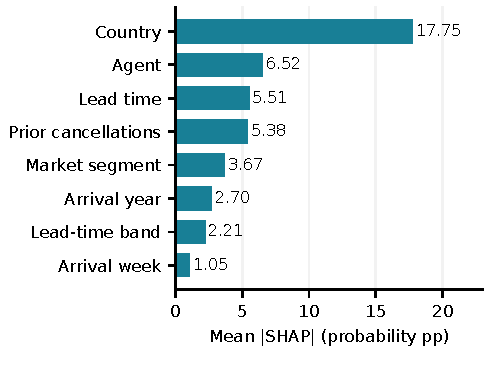
\includegraphics[width=\columnwidth]{forest_shap_single.pdf}
\caption{Grouped global SHAP importance for the fixed random-training forest. Units are probability percentage points. These explanations are specific to this estimator and sample.}
\label{fig:shap}
\end{figure}

The five largest mean absolute contributions are country (17.75 percentage points), agent (6.52), lead time (5.51), previous cancellations (5.38), and market segment (3.67). These explain the fitted model's score variation relative to its background; they do not estimate causal effects or the accuracy gained by adding each variable. Lead time and its band, calendar fields, stay components, and guest-composition features share information, which can divide attribution among correlated inputs. Interventional perturbations may also create combinations that are rare in actual bookings.

The numerical SHAP representation aligns tree thresholds with the forest's float32 routing without altering fitted trees or scores. Reconstructing probability as the background plus all feature contributions has maximum absolute error \(4.49\times10^{-8}\) across the 400 explained records. This confirms numerical reconstruction only. It does not validate calibration or prove that the explanation describes a feasible intervention.

\subsection{Individual Examples and Scope}
Two examples are chosen as the lowest and highest forest scores in the explanation sample, without selecting on outcome. Booking 3423 has a raw score near zero and outcome 0. Against a background of 37.38\%, its four largest absolute contributions are country ESP (\(-20.69\) percentage points), arrival year 2015 (\(-6.14\)), no previous cancellations (\(-4.10\)), and agent 38 (\(-3.77\)). Booking 75648 has a raw score near one and outcome 1; its largest terms are one previous cancellation (\(+34.90\)), country PRT (\(+20.61\)), lead time 290 days (\(+5.23\)), and arrival year 2015 (\(-4.27\)). The remaining terms are still needed for exact reconstruction.

These examples illustrate a decomposition, not typical predictive accuracy or certainty about an individual. Country and agent values encode context and may proxy policies, demand composition, or other unmeasured factors. They should not be treated as inherent guest characteristics or grounds for punitive decisions. The figures explain the random forest even if another classifier ranks better; they must not be relabelled as explanations of a boosted-tree model.
